%%%%%%%%%%%%%%%%%%%%%%%%%%%%%%%%%%%%%%%%%%%%%%%%%%%%%
%                                                   %
%     Penn State Colloquium Poster Template         %
%                                                   %
% Uses Penn State Colloquium class, with options:   %
%                                                   %
% Orientation:                                      %
%     portrait (default), landscape                 %
%                                                   %
% Paper size:                                       %
%     a4paper (default), a0paper, a1paper, a2paper, %
%     a3paper, a5paper, a6paper                     %
%%%%%%%%%%%%%%%%%%%%%%%%%%%%%%%%%%%%%%%%%%%%%%%%%%%%%
\documentclass{../psuposter}
\renewcommand{\templateimagepath}{../} 


%%%%%%%%%%%%%%%%%%%%%%%%%%%%%%%%%%%%%%%%%%%%%%%%%%%%%
%               Package Dependencies                %
%%%%%%%%%%%%%%%%%%%%%%%%%%%%%%%%%%%%%%%%%%%%%%%%%%%%%
\usepackage{natbib}
\usepackage{lipsum}                                % Dummy text
\usepackage[figwidth = 0.98\linewidth]{todonotes}  % Dummy image (and more!)
\usepackage[absolute, overlay]{textpos}            % Figure placement
\usepackage{braket}
\setlength{\TPHorizModule}{\paperwidth}
\setlength{\TPVertModule}{\paperheight}
\setcitestyle{numbers,square}


%%%%%%%%%%%%%%%%%%%%%%%%%%%%%%%%%%%%%%%%%%%%%%%%%%%%%
%                 AUTHOR AND TITLE                  %
%%%%%%%%%%%%%%%%%%%%%%%%%%%%%%%%%%%%%%%%%%%%%%%%%%%%%
\title{Exploring QCD Matter}
\author{Barbara Jacak}
\institute{UC Berkeley and Lawrence Berkeley National Laboratory}


%%%%%%%%%%%%%%%%%%%%%%%%%%%%%%%%%%%%%%%%%%%%%%%%%%%%%
%                  BEGIN DOCUMENT                   %
%%%%%%%%%%%%%%%%%%%%%%%%%%%%%%%%%%%%%%%%%%%%%%%%%%%%%
\begin{document}
\begin{frame}
\begin{columns}[t, totalwidth=\textwidth]
\begin{column}{0.45\textwidth - 1cm}


%%%%%%%%%%%%%%%%%%%%%%%%%%%%%%%%%%%%%%%%%%%%%%%%%%%%%
%                 BLOCK: BIOGRAPHY                  %
%%%%%%%%%%%%%%%%%%%%%%%%%%%%%%%%%%%%%%%%%%%%%%%%%%%%%
    \begin{block}{Speaker Biographic Summary}
    	\begin{center}
    		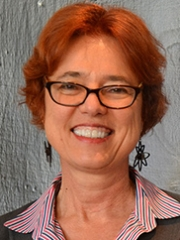
\includegraphics[width=0.5\textwidth]{images/portrait}
    	\end{center}
    	\href{}{Dr. Barbara Jacak} is a Professor of Physics at UC Berkeley and Director of the Nuclear Science Division at LBNL. She received her B.S at UC Berkeley and her Ph.D. at Michigan State University, where she did one of the first experiments at the K-500 Superconducting Cyclotron. Her research career includes 12 years at Los Alamos National Laboratory’s Physics Division, where she was a J. Robert Oppenheimer Fellow and scientific staff member. After that she spent 18 years as a Professor of Physics at Stony Brook University on Long Island in New York, including 6 years as Spokesperson of the PHENIX Collaboration at RHIC. Jacak is a Fellow of the American Physical Society, the American Association for the Advancement of Science, and the American Academy of Arts and Sciences. She is a member of the National Academy of Sciences, and serves as chair of the Academy’s Board on Physics and Astronomy.
    \end{block}


%%%%%%%%%%%%%%%%%%%%%%%%%%%%%%%%%%%%%%%%%%%%%%%%%%%%%
%            BLOCK: RESEARCH INTERESTS              %
%%%%%%%%%%%%%%%%%%%%%%%%%%%%%%%%%%%%%%%%%%%%%%%%%%%%%
    \begin{block}{Research Interests}
        Dr. Jacak’s research focuses on experimental study of quark gluon plasma. This formed in relativistic heavy ion collisions, where nuclei are heated to trillions of degrees and quarks are no longer confined inside hadrons. She is using fast quark and gluon probes of the plasma, following the fate of energy they lose as they traverse the plasma, in experiments at both CERN’s Large Hadron Collider and Brookhaven Lab’s Relativistic Heavy Ion Collider. 
        \begin{center}
	    	
\includegraphics[width=0.65\textwidth]{images/research}    		
	    	
	    	\textit{Distributions of unfolded asymmetries.} 
	    	\cite{acharyaTransverseMomentumDependent2021}
    	\end{center}

    	%\cite{longResearchLongLab}
    \end{block}
\end{column}
\begin{column}{0.55\textwidth - 1cm}


%%%%%%%%%%%%%%%%%%%%%%%%%%%%%%%%%%%%%%%%%%%%%%%%%%%%%
%                 BLOCK: ABSTRACT                   %
%%%%%%%%%%%%%%%%%%%%%%%%%%%%%%%%%%%%%%%%%%%%%%%%%%%%%
    \begin{block}{Talk Abstract}
    	Quantum Chromodynamics (QCD) predicts a transition from normal hadronic matter to a hot and/or dense phase where the quarks and gluons are no longer bound together and can move freely. Hot quark gluon plasmas with remarkable properties are produced in high energy collisions of heavy nuclei at the Relativistic Heavy Ion Collider (RHIC) in the U.S. and at the LHC in Europe.

		Vanishingly small shear viscosity to entropy density ratio means that they flow essentially without internal friction. Such plasmas are found to be very opaque to particles which experience the strong interaction. I will discuss how we probe transport properties of quark gluon plasma using hadron jets arising from quarks or gluons transiting the plasma. Small colliding systems may also produce a small droplet of quark gluon plasma, implying that it can emerge from the cold, dense gluonic matter deep inside nuclei within 1 fm/c. I will show how a future electron-ion collider will help address this question.
    \end{block}


%%%%%%%%%%%%%%%%%%%%%%%%%%%%%%%%%%%%%%%%%%%%%%%%%%%%%
%                BLOCK: BACKGROUND                  %
%%%%%%%%%%%%%%%%%%%%%%%%%%%%%%%%%%%%%%%%%%%%%%%%%%%%%
    \begin{block}{Brief Background}
    	Quark-Gluon plasma (QGP) is a state of strongly interacting matter, in which the quarks and gluons, which make up hadrons, are no longer confined to color-neutral entities of hadronic size. This can be achieved experimentally by colliding nuclear matter, especially via collisions of heavy ions. For example, typical collisions invovle ${}^{63}_{29}$Cu, ${}^{197}_{79}$Au, ${}^{238}{92}$U at RHIC and ${}^{208}_{82}$Pb at the LHC. The ultra-relativistic energies achieved in these colliders allow for the formation of a plasma in the laboratory that should be similar to the state of the primordial universe, in place up to a few microseconds after the Big Bang. \cite{maireIntroductionQuarkGluonPlasma2015}
    	%\cite{longLocalAxonalConduction2020} 
        \begin{center}
		   	
\includegraphics[width=0.75\textwidth]{images/background}    
		   	
		   	\textit{Depiction of Quark Gluon Plasma (QGP).}
		   	\cite{khalekScienceRequirementsDetector2021}
    	\end{center}
%		Second Paragraph 
		%\cite{longMorphologicalCharacterizationHVC2018} 
    \end{block}


%%%%%%%%%%%%%%%%%%%%%%%%%%%%%%%%%%%%%%%%%%%%%%%%%%%%%
%                 BLOCK: REFERENCES                 %
%%%%%%%%%%%%%%%%%%%%%%%%%%%%%%%%%%%%%%%%%%%%%%%%%%%%%
    \begin{block}{References}
        \bibliographystyle{aipnum4-1}
%        \bibliographystyle{iopart-num}
		\bibliography{references}
    \end{block}

\end{column}
\end{columns}


%%%%%%%%%%%%%%%%%%%%%%%%%%%%%%%%%%%%%%%%%%%%%%%%%%%%%
%                    FOOTER TEXT                    %
%%%%%%%%%%%%%%%%%%%%%%%%%%%%%%%%%%%%%%%%%%%%%%%%%%%%%
\begin{textblock}{0.5}(0.18, 0.94)
    \color{white}
    \sffamily
    \textbf{Eberly College of Science}
    \\
    Department of Physics
\end{textblock}


%%%%%%%%%%%%%%%%%%%%%%%%%%%%%%%%%%%%%%%%%%%%%%%%%%%%%
%                   END TEMPLATE                    %
%%%%%%%%%%%%%%%%%%%%%%%%%%%%%%%%%%%%%%%%%%%%%%%%%%%%%
\end{frame}
\end{document}
